\documentclass[a4paper,12pt]{article}
\usepackage[utf8]{inputenc}
\usepackage{graphicx} 
\usepackage{subfigure}
\usepackage[mathscr]{eucal}
\usepackage{titling}
\usepackage{float}
\usepackage{amsmath}
\usepackage{afterpage}
\usepackage{vmargin}
\usepackage[spanish]{babel}
\usepackage{eurosym} 
\usepackage{multirow} 
\usepackage{cite}
\usepackage{url}

\setpapersize{A4}	   %  DIN A4
\setmargins{3cm}    % margen izquierdo
{3.5cm}                     % margen superior
{15cm}                       % anchura del texto
{22.5cm}                   % altura del texto
{10pt}                         % altura de los encabezados
{1cm}                         % espacio entre el texto y los encabezados
{0pt}                           % altura del pie de página
{1cm}                         % espacio entre el texto y el pie de página

\begin{document}

\begin{titlepage}

\begin{center}
\vspace*{-1in}
\begin{figure}[htb]
\begin{center}

\includegraphics[width=8cm]{udc.eps}
\end{center}
\end{figure}

\vspace*{1in}
PROGRAMACIÓN DE SISTEMAS 20/21 Q1\\
\vspace*{1in}
\begin{Large}
\textbf{``Fagamos barullo''} \\
\end{Large}
\vspace*{3in}
\begin{large}
\raggedleft
\textbf{Autores:} Iñaki y Santiago \\
\textbf{Fecha:} \textit{A Coruña, Enero 2021}\\
\end{large}
\end{center}
\end{titlepage}
\addtocontents{toc}{\hspace{-7.5mm} \textbf{Capítulos}}
\addtocontents{toc}{\hfill \textbf{Página} \par}
\addtocontents{toc}{\vspace{-2mm} \hspace{-7.5mm} \hrule \par}
\pagenumbering{empty}
\tableofcontents
\thispagestyle{empty}
\newpage
\begin{flushright}
\begin{table}[hbtp]
\begin{center}
\caption{Tabla de versiones.}
\label{tabla:versiones}
\small
\vspace{1ex}
\begin{tabular}{|c|c|l|}
\hline
Versión & Fecha & Autor \\
\hline \hline
1.0 & 13/10/2020 & Iñaki y Santiago\\
2.0 & 29/10/2020 & Iñaki y Santiago\\
3.0 & 28/11/2020 & Iñaki y Santiago\\
4.0 & 23/12/2020 & Iñaki y Santiago\\
5.0 & 26/01/2020 & Iñaki y Santiago\\
\hline
\end{tabular}
\end{center}
\end{table}
\end{flushright}
\thispagestyle{empty}
\newpage
\pagenumbering{arabic}
\section{Introducción}
\subsection{Objetivos}
Desarrollar una aplicación para encontrar integrantes para bandas emergentes locales de una forma rápida y sencilla. Nos centraremos en crear una aplicación con una experiencia de usuario al nivel del 2020 y que cumpla con las expectativas de los usuarios ---es decir, que les ayude realmente a encontrar músicos para sus bandas---.

También, la aplicación servirá para que promotores, u organizadores de eventos, puedan encontrar bandas locales y prometedoras con ganas de pisar un escenario por primera vez.
\subsection{Motivación}
Encontrar integrantes para un nuevo grupo es muy difícil. Si alguna vez te has visto en esta situación, te habrás dado cuenta de que no importa cuántos carteles cuelgues en las salas de ensayos locales, ni siquiera cómo de llamativos sean. Todos tus esfuerzos serán en vano y tu cartel será completamente ignorado. Además, si eres nuevo en la ciudad, o simplemente estás empezando en el mundo de la música, vas a tener pocos contactos en tu agenda de los que poder depender.

Otra opción son las páginas de anuncios en línea, como por ejemplo \url{https://www.milanuncios.com}. Sin embargo, estas páginas tampoco son una buena opción. Los anuncios de grupos que buscan integrantes rápidamente quedan tapados por otros más atractivos ---guitarras que se venden por ejemplo--- que generan más visitas y se acaban posicionando de primeros en los resultados de búsqueda.

Por último, promocionar una banda es igual o más difícil que montarla. 
Por eso, queremos desarrollar una aplicación sencilla y eficaz que ayude a bandas emergentes a empezar a despegar en el mundo de la música.
\subsection{Trabajo relacionado}
Sin duda existen ya infinidad de aplicaciones que ayudan a músicos a encontrar bandas. Además, ahora que las redes sociales son prácticamente el CV del siglo XXI, casi cualquier página sería competidora de nuestra aplicación. Sin embargo, creemos que tenemos potencial por encima de estas plataformas, ya que ofrecemos una funcionalidad muy específica que ayuda a empezar y a promocionar bandas locales de forma sencilla y directa.
\section{Análisis de requisitos}
\subsection{Funcionalidades}
Queremos que nuestra aplicación registre dos perfiles de usuario: músico y promotor. Con el perfil de músico creado, podemos proceder a: buscar bandas locales que necesitan integrantes o crear nuestra propia banda y crear un anuncio para encontrar integrantes.

En cuanto al proceso de búsqueda de bandas, cada músico verá solo las bandas que buscan músicos con su perfil. Es decir, bandas que buscan los instrumentos que sepa tocar el usuario. Además, también será posible explorar bandas locales.

Para que los músicos destaquen, podrán personalizar su perfil con fotos y varias maquetas con las que demuestren su habilidad. También será posible valorar positivamente el perfil de un músico para que aparezca por encima del resto en las búsquedas locales. De la misma forma, las bandas podrán editar su perfil para venderse de forma más atractiva a los promotores y podrán recibir valoraciones positivas.
\subsection{Prioridades}
La prioridad número uno es desarrollar una versión dónde se puedan registrar los músicos y poder ver a los músicos de tu zona atendiendo a una serie de filtros (instrumento, edad, etc.). Tendrán un perfil básico con fotos, maquetas e información personal y de contacto.

En una fase posterior, la aplicación podrá registrar bandas, que son agrupaciones de uno o más músicos. El perfil de banda contiene fotos, alguna maqueta e información básica. Además, como con los músicos, también será posible explorar bandas. Podremos filtrar la búsqueda con filtros como el género, faltan integrantes, etc.

Por último, aparecería el perfil de promotor. Este perfil puede explorar bandas y músicos con el fin de contactar con ellos para ofrecer contratos de grabación, conciertos, etc.
\section{Planificación inicial}
\subsection{Iteraciones}
\subsubsection{Iteración 1: registro y persistencia}
Desarrollar una aplicación sencilla dónde podamos registrar músicos. También podremos identificarnos, por lo que tiene que existir persistencia.
\subsubsection{Iteración 2: perfil músico}
Al final de esta iteración podremos acceder a nuestro perfil y editarlo. Podremos modificar información de contacto y personal, fotos y maquetas.
\subsubsection{Iteración 3: explorar músicos}
En esta iteración implementaremos la funcionalidad de poder buscar otros músicos ---pudiendo hacer uso de filtros--- y acceder a sus perfiles. Además, podremos valorar sus perfiles positivamente.
\subsubsection{Iteración 4: crear grupos}
Se podrán crear bandas, editar su información y buscarlas. Existirá un filtro de búsqueda especial con el que encontrar bandas que busquen integrantes.
\subsubsection{Iteración 5: promotores}
Se introduce el perfil de promotor que podrá explorar bandas locales emergentes.
\subsection{Responsabilidades}
Por preferencia, Santiago prefiere el \textit{front-end}, con un perfil especializado en la usabilidad y el desarrollo orientado al \textit{testing} e Iñaki el \textit{back-end}, ya que le parece un reto y le gusta ponerse a prueba diseñando arquitecturas sencillas y eficientes. Sin embargo, seremos flexibles y podremos ayudar el uno al otro. Idealmente descompondremos cada iteración en pequeñas tareas y trabajaremos de acuerdo a la filosofía \textit{Git Flow}.
\subsection{Hitos}
\subsubsection{Hito 1: explorar músicos}
Como ya comentamos en el análisis de requisitos, lo más importante de la aplicación es poder buscar a otros músicos. Por eso, fijamos un hito que será una versión de la aplicación con la que podremos registrarnos y buscar perfiles locales.

Programaremos el registro, el \textit{login}, la búsqueda y la edición y visualización de perfiles. Haremos tests de unidad cuando sea necesario y testeo de interfaz para comprobar que todos los casos de uso de este hito funcionan correctamente.
\subsubsection{Hito 2: explorar bandas}
El segundo hito de nuestro proyecto, será tener una aplicación en la que podamos crear bandas y anuncios para encontrar integrantes. De esta forma, tendremos una experiencia más rica a la hora de interactuar con la aplicación y no nos limitaremos únicamente a ver perfiles de otros músicos.

Programaremos la creación de grupos, la edición de bandas y la búsqueda local. De nuevo, haremos tests unitarios y probaremos los casos de uso comprobando que todo fluye correctamente.
\subsubsection{Hito 3: promotores}
Por último, aparecerá el rol de promotor que podrá explorar bandas y obtener su información de contacto para contratarlas, etc.

Una vez más, probaremos las unidades que sean necesarias y probaremos los casos de uso relacionados.
\subsection{Incidencias}
No seguiremos un plan de gestión de riesgos. Sin embargo, seremos cuidadosos y si encontramos un problema que ponga en riesgo el transcurso del proyecto, contactaremos con los profesores para obtener alternativas y soluciones.
\subsubsection{Indicendia 1: \textit{back-end} y capa de acceso a servicios}
El \textit{back-end} es un hueso importante de la aplicación. Es imprescindible poder comunicarnos con un servidor para poder acabar la iteración 1.

En un primer momento pensamos en desarrollar un \textit{back-end} pequeño usando entornos de desarrollo sencillos y con una curva de aprendizaje pequeña (i.e. Python Flask). Sin embargo, nos dimos cuenta de que también necesitamos crear la capa de acceso a servicios en el código \textit{Java}. Entonces, decidimos resolver el problema usando Firebase. Así, no tendremos que implementar el servidor remoto ni la capa de acceso a servicios y nos podremos centrar en lo que importa: que la aplicación funcione.
\section{Estado actual}
Hito 1 cumplido (Iteraciones 1, 2 y 3). La aplicación es completamente funcional y resuelve el objetivo principal: poder encontrar integrantes para bandas emergentes locales. Además, tiene una interfaz de usuario moderna y sigue los mejores principios de usabilidad (ver fotos del anexo).

Concretamente, la apliación permite registrarnos para poder acceder al servicio. Desde ahí, podemos visualizar nuestro perfil y editarlo (descripción, instrumentos, fotos y maquetas). Por último, podemos buscar y ver el perfil de otros usuarios filtrandolos por nombre, instrumentos y ``favoritos''.
\section{Diseño}
\subsection{Arquitectura}
Seguiremos el modelo MVVP visto en clase para desarrollar la aplicación por capas. Las actividades representarán las vistas y el \textit{presenter} las engranará con la lógica de negocio (i.e. el modelo). Así conseguiremos responsabilidades únicas y podremos trabajar por interfaces. Lo que hace que el reparto de tareas sea más sencillo y se pueda ajustar más al perfil de cada desarrollador.
\subsubsection{Vistas}
Las vistas son las encargadas de mostrar por pantalla la información al usuario. En el caso de Android, las vistas se implementan a través de Actividades. Hasta el momento, la aplicación se compone de nueve actividades (ver cuadro \ref{tab:actividades}) y tres fragmentos (ver cuadro \ref{tab:fragmentos}).
\begin{table}[tt]
	\centering
	\label{tab:actividades}
	\caption{Actividades de la aplicación.}
	\begin{tabular}{|l|l|}
		\hline
		Actividad & Descripción \\
		\hline \hline
		\texttt{SplashScreen}* & Punto de entrada\\ \hline
		\texttt{Register} & Implementa la lógica de registro\\ \hline
		\texttt{Login} & Implementa la lógica de login\\ \hline
		\texttt{MainActivity} & Landing page (una vez identificado)\\ \hline
		\texttt{ProfileSettings} & Lógica para modificar nuestro perfil\\ \hline
		\texttt{AccountSettings} & Lógica para modificar la cuenta\\ \hline
		\texttt{Licenses} & Licencias de librerías de terceros\\ \hline
		\texttt{AddPhoto} & Lógica para añadir una foto\\ \hline
		\texttt{AddMp3} & Lógica para añadir una maqueta\\ \hline
	\end{tabular}
	
	\vspace{2mm}
	(*) Es la actividad principal de la aplicación y punto de entrada que vemos en el launcher de Android. Esta actividad nos redirige a \texttt{MainActivity} si ya estamos identificados o a \texttt{Register} en el caso contrario.
\end{table}

\begin{table}[t]
	\centering
	\label{tab:fragmentos}
	\caption{Fragmentos de la aplicación.}
	\begin{tabular}{|l|l|}
		\hline
		Fragmento & Descripción \\
		\hline \hline
		\texttt{Profile} & Muestra información de un usuario\\ \hline
		\texttt{Search} & Implementa la lógica de búsqueda\\ \hline
		\texttt{Settings} & Punto de entrada al resto de ajustes\\ \hline
	\end{tabular}
\end{table}

La actividad \texttt{SplashScreen} es el punto de entrada a la aplicación. Se encarga de determinar si ya estamos identificados o no. En el caso de estarlo nos redirige a la \texttt{MainActivity}, sino a la actividades \texttt{Register} o \texttt{Login}.

Las actividades \texttt{Register} y \texttt{Login} son las encargadas de, respectivamente, ofrecer la funcionalidad de registro e identificación. Son triviales, ya que no presentan ningún elemento complejo.

Por otro lado, la activiadad \texttt{MainActivity} es algo más compleja. Esta actividad es la página de entrada a la aplicación cuando nos hemos identificado. Tiene una \textit{NavigationBar} que nos permite movernos por tres pestañas distintas: mi perfil, búsqueda de usuarios y ajustes. Estas pantallas están implementadas como \textit{Fragments}\footnote{De esta forma se pueden reusar en la aplicación. En concreto, el fragmento de \texttt{Profile} se usa indistintamente para mostrar información sobre nuestro perfil y el de otros usuarios.} (\texttt{Profile}, \texttt{Search} y \texttt{Settings}) y con un controlador por cada uno de ellos\footnote{También podíamos haber usado un \textit{mega-presenter}, con el que probablemente se hubiese podido reusar código entre las vistas. Sin embargo, el problema de esta aproximación es que hay que crear más interfaces entre los fragmentos y propagar los resultados entre más vistas, lo que añade complejidad de forma innecesaria.}.

En cuanto al resto de actividades, de nuevo, son triviales. Implementan la funcionalidad que indica el cuadro \ref{tab:actividades} de forma sencilla e intuitiva para el usuario.
\subsubsection{Controladores}
Uno por cada vista descrita en la subsección anterior. Unen la vista con la lógica de negocio (i.e. modelo). De esta forma, conseguimos que las actividades simplemente gestionen lo relacionado con la vista y que el modelo solo implemente la lógica de negocio. Estas clases simplemente transforman los flujos de datos para que, tanto las vistas como los modelos, reciban únicamente los datos que les interesan.
\subsubsection{Modelo}
En este caso, la lógica de negocio se encarga de: la autenticación y el almacenamiento de información sobre usuarios en la red. A su vez, se divide en dos capas distintas: los servicios ---que implementan la lógica propiamente dicho--- y los \textit{datasources}, que abstraen el acceso a los datos (tanto si son por red, al almacenamiento local, etc.).

Su implementación no tiene mayor relevancia ---llamadas entre capas y se usan las librerías de Firebase para acceder a la red---. Por lo que nos limitaremos a comentar los datos que usamos en nuestra lógica de negocio para implementar la funcionalidad de la aplicación. En cuanto al servicio de autenticación, guardamos los siguientes datos para un usuario
\begin{table}[H]
	\centering
	\begin{tabular}{|l|l|l|}
		\hline
		\texttt{Email}* &
		\texttt{Password} &
		\texttt{UID} \\
		\hline
	\end{tabular}
\end{table}

Sobre cada usuario se guarda la siguiente información
\begin{table}[H]
	\centering
	\begin{tabular}{|l|l|l|l|l|}
		\hline
		\texttt{UID}* &
		\texttt{Full name} &
		\texttt{Phone number} &
		\texttt{Profile pic} &
		\texttt{Instruments}\\
		\hline
	\end{tabular}
\end{table}

Además, también se guarda la relación de perfiles favoritos
\begin{table}[H]
	\centering
	\begin{tabular}{|l|l|}
		\hline
		\texttt{Following}* &
		\texttt{Follower}*\\
		\hline
	\end{tabular}
\end{table}

Fotos
\begin{table}[H]
	\centering
	\begin{tabular}{|l|l|l|l|}
		\hline
		\texttt{FID}* &
		\texttt{UID} &
		\texttt{PhotoBlob} &
		\texttt{PhotoTitle}\\
		\hline
	\end{tabular}
\end{table}

Y maquetas
\begin{table}[H]
	\centering
	\begin{tabular}{|l|l|l|l|l|}
		\hline
		\texttt{DID}* &
		\texttt{UID} &
		\texttt{DemoBlob} &
		\texttt{DemoPhotoBlob} &
		\texttt{DemoTitle}\\
		\hline
	\end{tabular}
\end{table}
\subsection{Interfaces de usuario}
Las interfaces de usuario siguen las mejores prácticas de las guías de diseño de \textit{Material Design}. De esta forma, la aplicación ofrece una interfaz agradable y sencilla con una buena experiencia de usuario (ver anexo de figuras).
\subsection{Pruebas}
\subsubsection{Pruebas de interfaz}
Se han programado \textit{UITests} con el \textit{framework} Espresso para llevar al límite los casos de uso \texttt{Register} y \texttt{Login} y comprobar si funciona todo correctamente ---también permiten comprobar que la aplicación es robusta, ya que los datos se validan antes de enviarlos al servidor---. Además, también se ha probado la aplicación manualmente para comprobar que la navegación es consistente (i.e. cuando te identificas no puedes volver para atrás).

\vspace{.5cm}
\noindent
{\centering
\fbox{\parbox{\dimexpr.978125\textwidth}{\textbf{Nota:} Sería interesante poder automatizar la ejecución de las pruebas de unidad e interfaz con las \textit{pipelines} de GitLab. De este modo, cuando se empujase un \textit{commit} al repositorio, se notificaría al desarrollador de si los cambios han pasado los \textit{tests} de forma satisfactoria o no. De este modo, podríamos realizar un desarrollo orientado a pruebas en el que primero programásemos los \textit{tests} y después los casos de uso.}}}
\subsection{Librerías de terceros}
Todas las licencias están correctamente embebidas en la actividad \texttt{Licenses} para cumplir con las condiciones de uso del \textit{software}.
\subsubsection{Picasso}
Permite gestionar la descarga de imágenes de forma sencilla y se encarga de \textit{cachear} resultados automáticamente, liberándonos de gran parte de la gestión con el sistema de ficheros de Android.
\subsubsection{Butter Knife}
Gestiona la asociación de \textit{widgets} a variables automáticamente. Permite eliminar gran parte del \textit{boilerplate} necesario para poder trabajar con las actividades.
\subsubsection{FlexboxLayout}
Es una librería que permite usar un \textit{layout} similar al \textit{CSS Flexible Box Layout} en Android. De esta forma, no tenemos que preocuparnos de gestionar vistas complejas en la que los elementos se mueven y tienen que estar perfectamente centrados.
\section{Trabajo futuro}
Con el estado actual de la aplicación, sería sencillo acabar con los hitos 2 y 3. De esta forma, la aplicación podría pasar a usarse en una ciudad ---i.e. Pontevedra--- para que músicos jóvenes puedan formar una banda, empezar a ensañar en el local de música del \textit{concello} y fácilmente conseguir ``bolos'' al ser descubiertos por promotores, sin necesidad de anunciarse por la ciudad o yendo de puerta en puerta.
\section*{Anexo de figuras}
\addcontentsline{toc}{section}{Anexo de figuras}
\begin{figure}[H]
	\centering
	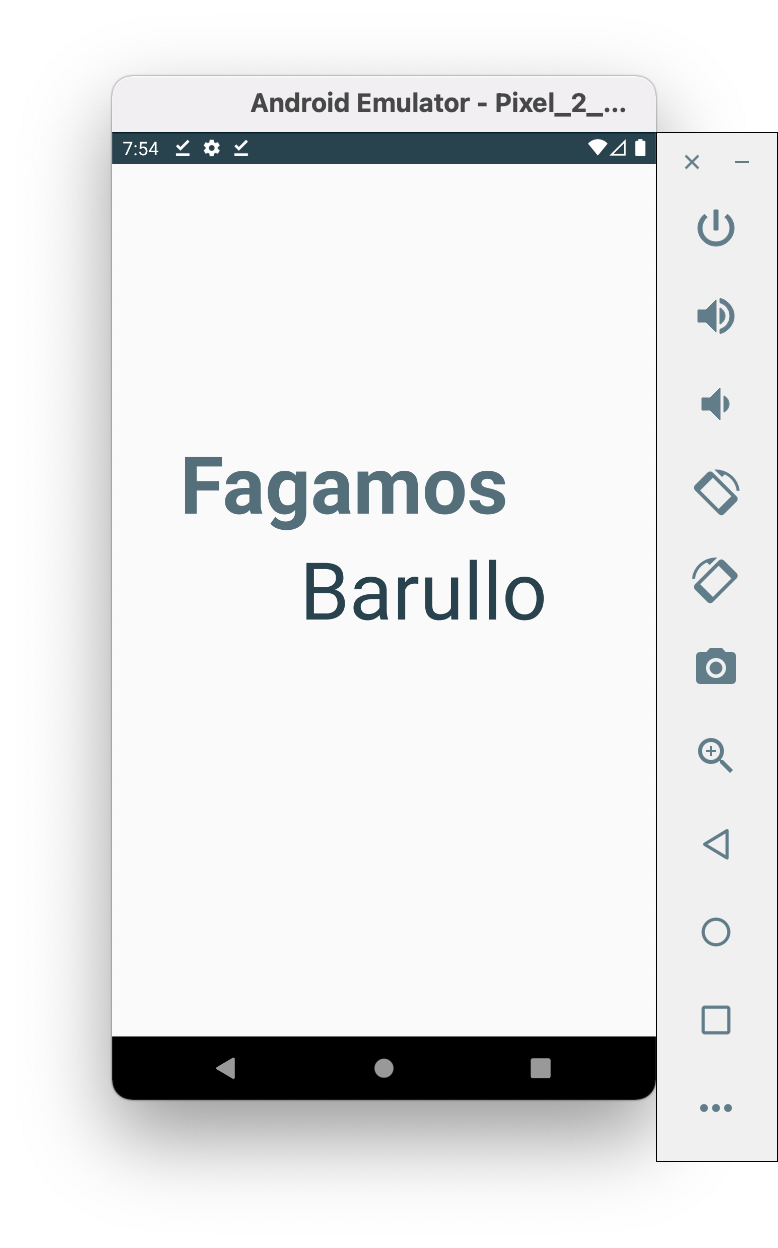
\includegraphics[scale=.42]{1.png}
\end{figure}
\begin{figure}[H]
	\centering
	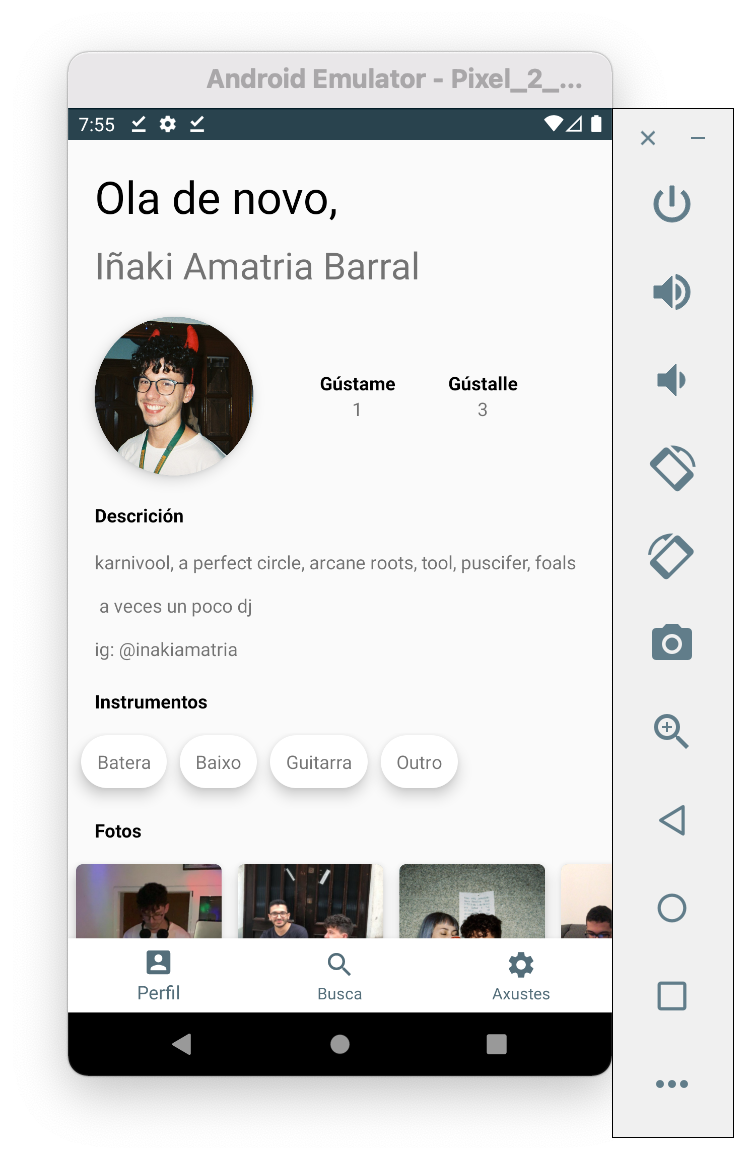
\includegraphics[scale=.42]{2.png}
\end{figure}
\begin{figure}[H]
	\centering
	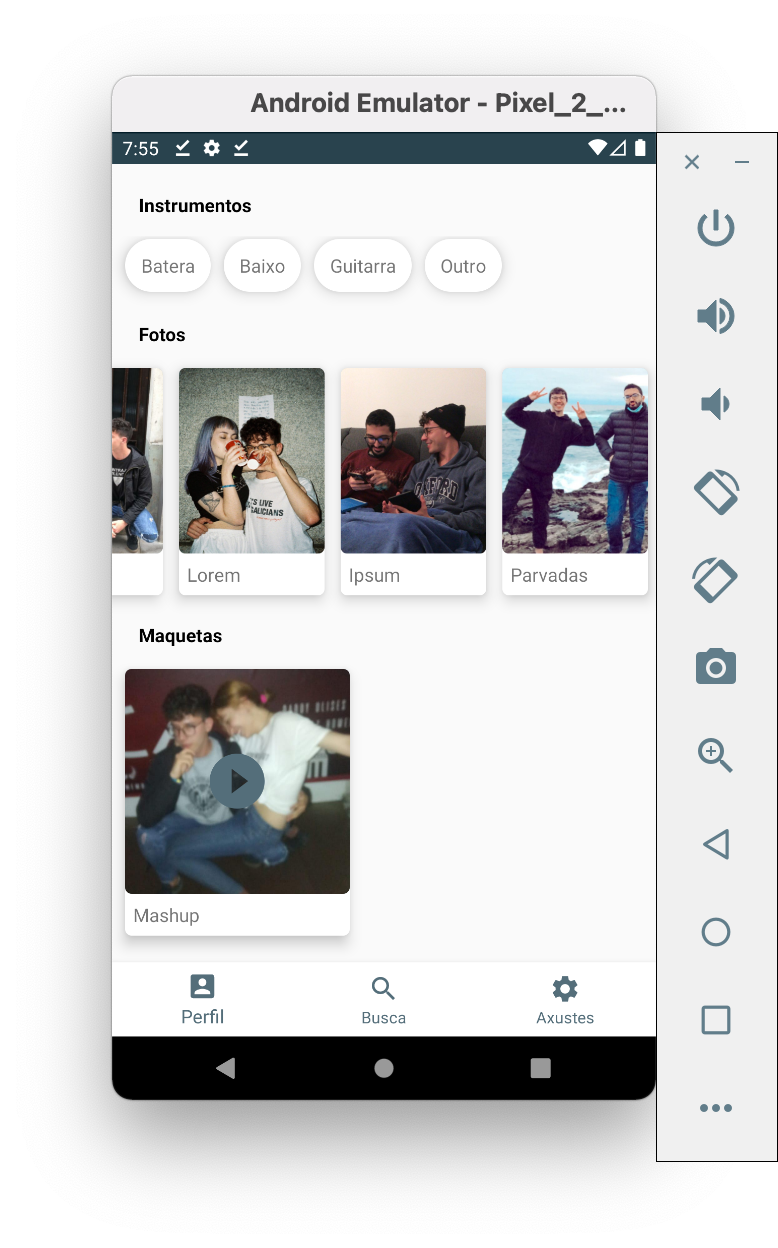
\includegraphics[scale=.42]{3.png}
\end{figure}
\begin{figure}[H]
	\centering
	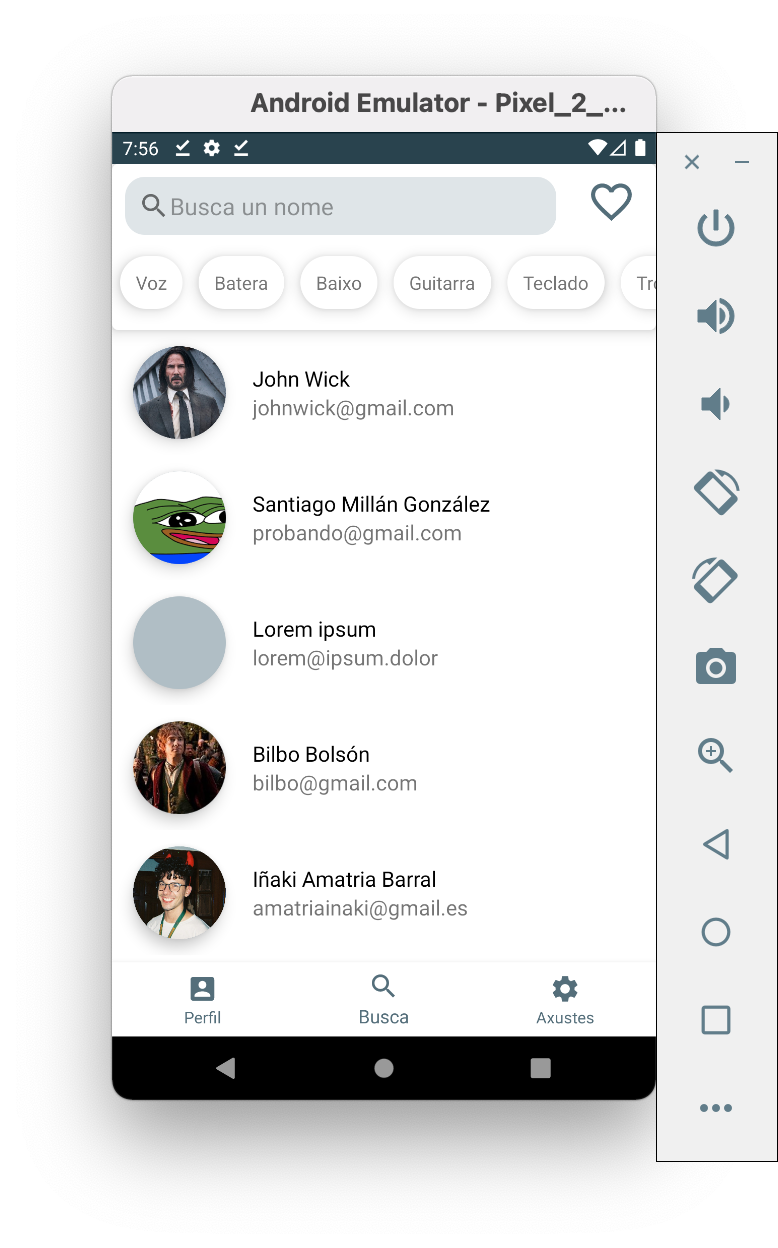
\includegraphics[scale=.42]{4.png}
\end{figure}
\begin{figure}[H]
	\centering
	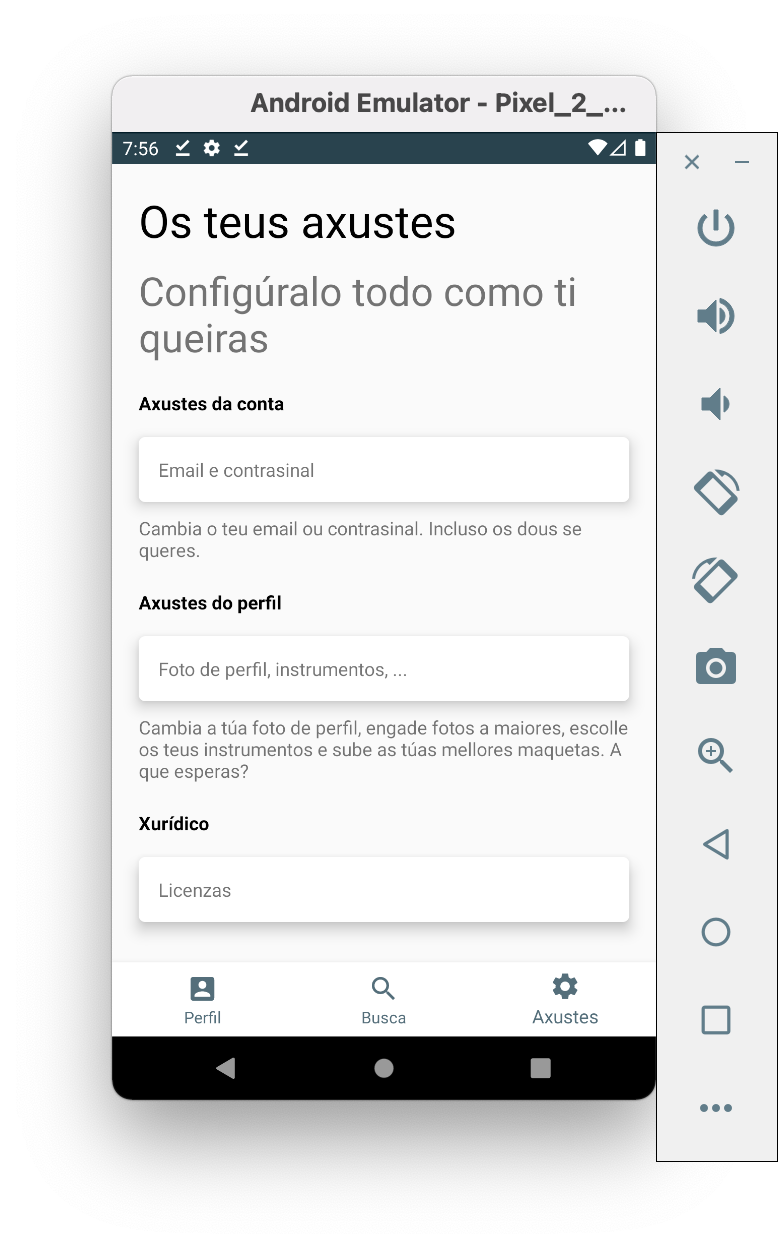
\includegraphics[scale=.42]{5.png}
\end{figure}
\begin{figure}[H]
	\centering
	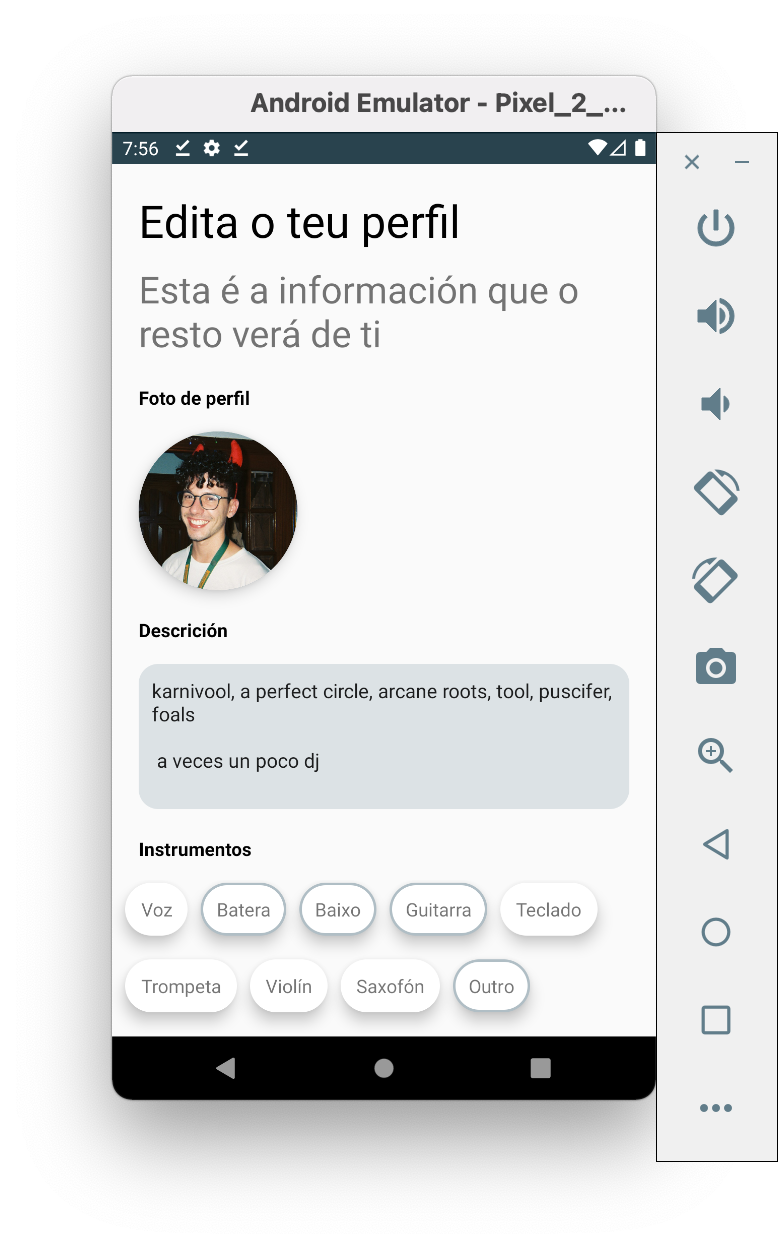
\includegraphics[scale=.42]{6.png}
\end{figure}
\begin{figure}[H]
	\centering
	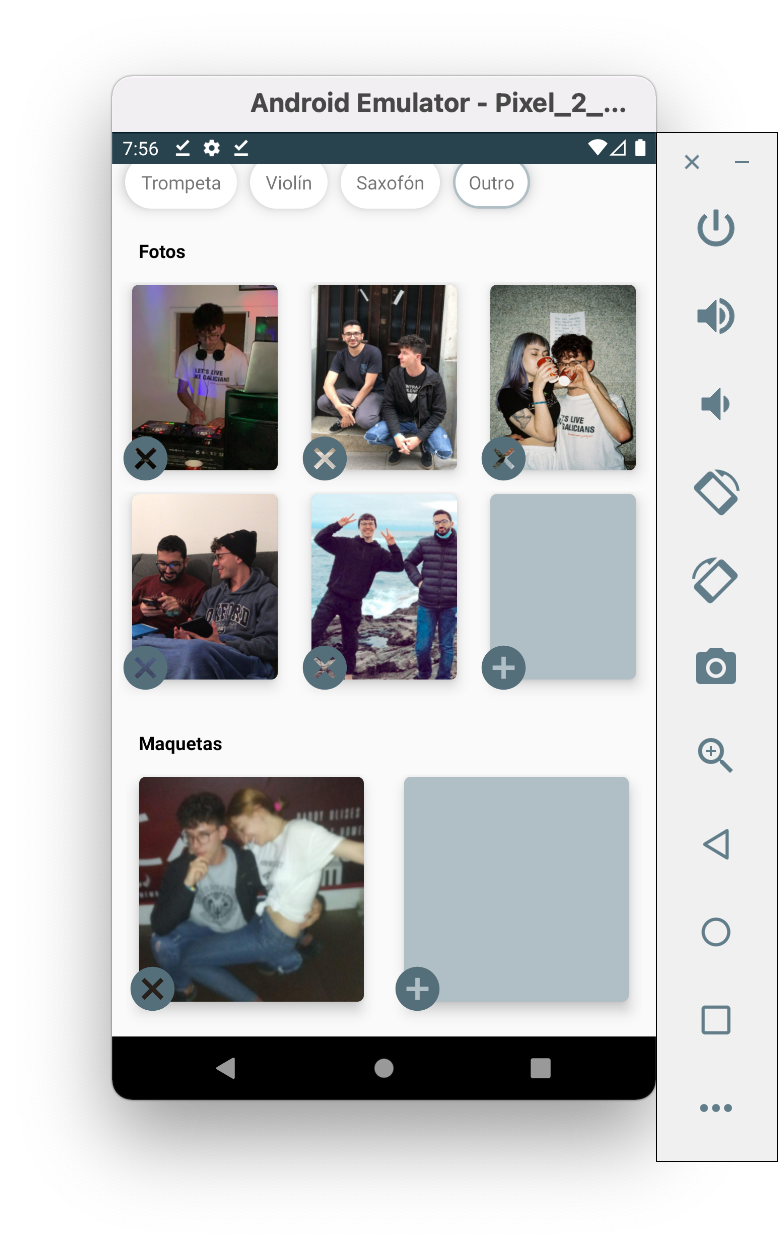
\includegraphics[scale=.42]{7.png}
\end{figure}
\begin{figure}[H]
	\centering
	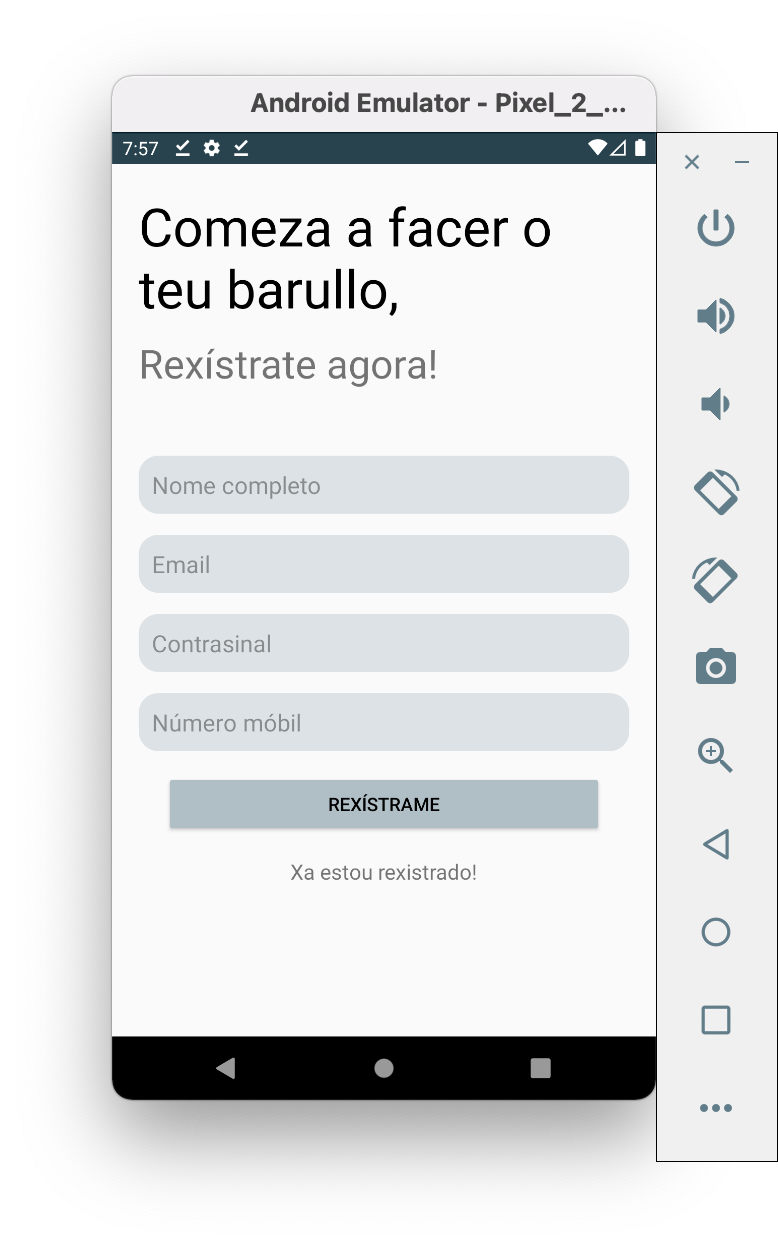
\includegraphics[scale=.42]{8.png}
\end{figure}
\begin{figure}[H]
	\centering
	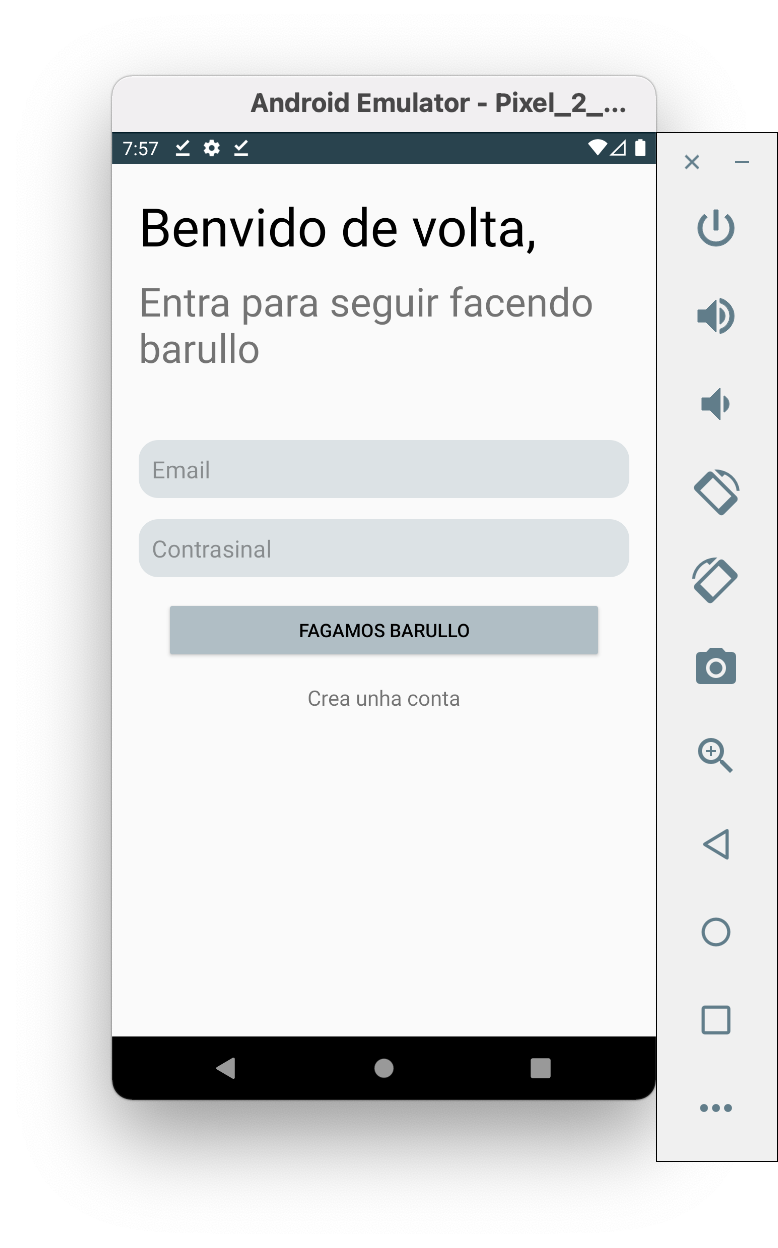
\includegraphics[scale=.42]{9.png}
\end{figure}
\end{document}